\section{\textsc{Источники ошибок GPS}}

Многочисленные физические эффекты вносят свой вклад в точность измерений GPS. 
Источники ошибок GPS можно сгруппировать в три категории, которые связаны с: спутником, распространением сигнала и приёмником.
В табл. \ref{tab-errors} приведена такая классификация несколько наиболее важных источников ошибок GPS. 
С другой стороны, ошибки можно разделит на систематические (biases) и случайные. 
Большинство ошибок GPS являются систематическими, включая атмосферные эффекты, эффект многолучёвости и сдвиг фазового центра антенны приёмника. 
Основным источником случайных ошибок является шум приёмника, его наиболее трудно прогнозировать и моделировать.
\begin{table}[h]
\caption{\centerline{Классификация источников ошибок GPS.}}
\label{tab-errors}
\centering
\begin{tabular}{|c|c|}
\hline
Категория               & Источник ошибки                                                                                                              \\ \hline
Спутник                 & \begin{tabular}[c]{@{}c@{}}Ошибка часов\\ Ошибки эфемерид\end{tabular}                                                       \\ \hline
Распространение сигнала & \begin{tabular}[c]{@{}c@{}}Ионосферные эффекты\\ Тропосферные эффекты\end{tabular}                                           \\ \hline
Приёмник                & \begin{tabular}[c]{@{}c@{}}Ошибка часов\\ Эффект многолучёвости\\ Cдвиг фазового центра антенны\\ Шум приёмника\end{tabular} \\ \hline
\end{tabular}
\end{table}

Ошибки GPS могут быть учтены при помощи параметров коррекции или устранены с использованием различных методов позиционирования.
Параметры коррекции, например, могут передаваться в навигационном сообщении, предоставляться службой IGS или рассчитываться атмосферными моделями.
Однако они учитывают только определённую часть ошибок.
Например, модель Клобучара устраняет около половины вклада ионосферных ошибок. 
Параметры часов и эфемерид доступны с различной степенью точности.
Кроме того, благодаря комбинации метода относительного позиционирования и двухчастотных приёмников, некоторые ошибки могут быть устранены полностью.
Например, разность измерений двух приёмников может полностью устранить ошибки, связанные со спутником, а разность измерений двух спутников -- ошибки приёмника.
Метод двойных разностей (double difference), т.е. с участием двух приёмников и двух спутников, может эффективно использоваться для устранения всех аппаратных ошибок.
Далее, кратко рассмотрим основные источники ошибок GPS.

\subsection*{\textbf{Ошибки часов и эфемерид}}

Смещение, дрейф и скорость дрейфа часов каждого спутника GPS передаётся в навигационном сообщении.
Эта информация представлена в виде коэффициентов полинома 2-ой степени:
\begin{equation}
\delta^s=a_0+a_1(t-t_0)+a_2(t-t_0)^2
\end{equation}
где 
$t_0$ -- эталонная эпоха; 
$a_0$, $a_1$ и $a_2$ -- смещение, дрейф и скорость дрейфа часов спутника.
Их типичные значения: $a_0<1\,\text{мкс}$, $a_1\approx10^{-11}$ и $a_2\approx0\,\text{c}^{-1}$ \cite{Seeber2003}.
Сегмент управления GPS постоянно отслеживает эти параметры и каждые два часа отправляет их обновленные значения всей группировке спутников. 
Эталонная эпоха $t_0$ соответствует последнему времени обновления. 
Такие параметры обычно устраняют ошибку часов спутника в переделах 5 нс.
Более точные параметры, например от IGS, могут повысить точность до 75 пс ($75\times10^{-12}$ с).

Атомные часы стоят дорого, поэтому многие приёмники GPS используют более дешёвые альтернативные варианты, такие как кварцевые часы.
Однако кварцевые часы менее стабильны, чем атомные.
Величина их дрейфа составляет порядка от $10^{-10}$ до $10^{-8}$. 
Не смотря на это, приёмник GPS может сам оценить сдвиг и дрейф собственных часов.
На основе этих оценок, он использует определённые методы их устранения \cite{Petovello2011}. 
Один из таких методов ``управляет'' генератором часов, непрерывно сводя дрейф к нулю.
Это поддерживает постоянное смещение времени в пределах уровня шума, что обеспечивает его простую коррекцию.  
Второй (более распространённый) метод позволяет приёмнику вводить дискретные скачки времени, чтобы устранить накопленное смещение.
Смещение часов приёмника может быть оценено и компенсировано с точность до 1 мкс, что соответствует ошибке измерения дальность около 300 м. 
Эта ошибка, очевидно, неприемлема для подавляющего большинства приложений GPS, поэтому необходимо использовать методы для устранения остаточного смещения.
Как правило, ошибка часов приёмника $\delta_r$ включается неизвестной в уравнения измерений.
Также можно использовать разностные методы.

Эфемериды спутников, передаваемые в навигационном сообщении, могут незначительно отличаться от истинных параметров орбит.
Более точные эфемериды предоставляются различными службами ГНСС, включая IGS.
В прошлом ошибки широковещательных эфемерид приводили к нескольким метрам ошибки позиционирования.
Для решения этой проблемы были предприняты многочисленные усилия, которые в значительной степени оказались оправданными.
В отчёте за 2012-2013 годы было установлено, что созвездие GPS имеет среднее значение SISRE (Signal In Space Ranging Error), равное 0,7 м \cite{Montebruck2015}.  
Для коротких базовых линий также можно использовать метод дифференциального позиционирования.

\subsection*{\textbf{Релятивистские эффекты}}

Эффект замедления времени из-за специальной теории относительности вызывает отклонение номинальной частоты сигнала \cite{Hofmann2008}:
\begin{equation}
\frac{f_0^{'}-f_0}{f_0}=-4,464\times10^{-10}    
\end{equation}
Это отклонение выглядит несущественным, но эффект накапливается, поэтому вносимая ошибка становится большой.
Можно оценить на сколько часы спутника будут дрейфовать относительно часов на Земле в течение одного дня: $-4,464\times10^{-10}\times60\times60\times24\approx-38,6$ мкс/день.
Эта временная задержка, умноженная на скорость света в вакууме $c$, соответствует ошибке расстояния, равной 11,6 км/день. 

Вращение Земли тоже вызывает ошибку, которую необходимо учитывать. 
В геоцентрической инерциальной системе координат вращение учитывается через ``коррекцию пути'', которая определяется движением приёмника между передачей и приёмом сигнала:
\begin{equation}
\Delta\rho=\frac{(\vec{r}_r-\vec{r^s})\cdot\vec{v}_r}{c}    
\end{equation}
где
$\vec{r}_r$ и $\vec{r^s}$ -- геоцентрические радиус-векторы приёмника и спутника;
$\vec{v}_r$ -- вектор скорости приёмника (учитывает скорость из-за вращения Земли и кинематическую скорость относительно поверхности Земли). 
Величина коррекции пути может составлять до 30 м \cite{Hecimovic2013}.  

Дополнительные релятивистские эффекты, которые связаны с эксцентриситетом орбиты спутника и искривлением пространства-времени (общей теорией относительности) достаточно малы, поэтому в большинстве случаев ими можно пренебречь. 

\subsection*{\textbf{Wind-up эффект}}

Wind-up эффект влияет только на измерения фазы несущей и возникает в волнах с круговой поляризацией.
Так как все сигналы GPS имеют правую круговую поляризацию, то wind-up эффект, который хоть и невелик, должен быть учтён. 
Этот эффект зависит от относительной ориентации антенн спутника и приёмника, а также от вектора линии видимости (Line Of Sight, LOS) между ними.
Суть эффекта заключается в следующем.
Когда спутник вращается вокруг Земли, он должен постоянно переориентироваться, чтобы его солнечные панели получали максимум энергии от Солнца.
Это вращение создает изменение фазы, которое приёмник интерпретирует, как изменение расстояния. 

\subsection*{\textbf{Атмосферные эффекты}}

Как ионосферные, так и тропосферные эффект оказывают влияние на точность позиционирования GPS, но в данной работе более подробно будут рассмотрены только первые из них (см. ГЛАВА 2. Ионосфера и её влияние на сигналы GPS). 

\subsection*{\textbf{Эффекты многолучёвости, дифракции и интерференции}}

Эффект многолучёвости возникает, если сигнал от спутника к приёмнику приходит несколькими разными оптическими путями (например, из-за отражения).
Как правило, прямой и отражённый сигнал приходят на приёмник в немного разное время из-за разной длины пути, как показано на рис. \ref{fig-signal-paths} (a).
В некоторых случаях прямой сигнал может быть полностью перекрыт, тогда на приёмник приходит только отражённый сигнал, как показано на рис. \ref{fig-signal-paths} (b).
Длина пути отражённого сигнала больше, чем прямого.
Это приводит к ошибке позиционирования приёмника.
Ошибка многолучевого распространения при использовании псевдодальности, как правило, составляет около 10-20 м \cite{Wells1987}, хотя в отдельных случаях может достигать 100 м \cite{VanNee1992}.
Ошибка многолучевого распространения при измерениях фазы несущей намного меньше и обычно составляет не более 1 см \cite{Hofmann2008}. 
Общей аналитической модели многолучевого распространения не существует, т.к. эффект многолучёвости сильно зависит от местности и угла прихода сигнала, который меняется при движении спутника. 
При наличии нескольких отражателей, например, как в плотной городской среде, многолучевое распространение становится слишком сложным и моделируется статистически \cite{Rappaport2002}. 
Также для устранения эффекта многолучёвости можно использовать приёмные антенны специальной конструкции (например, дроссельные кольцевые антенны) или метод дифференциального позиционирования.
\begin{figure}[h]
\centering    
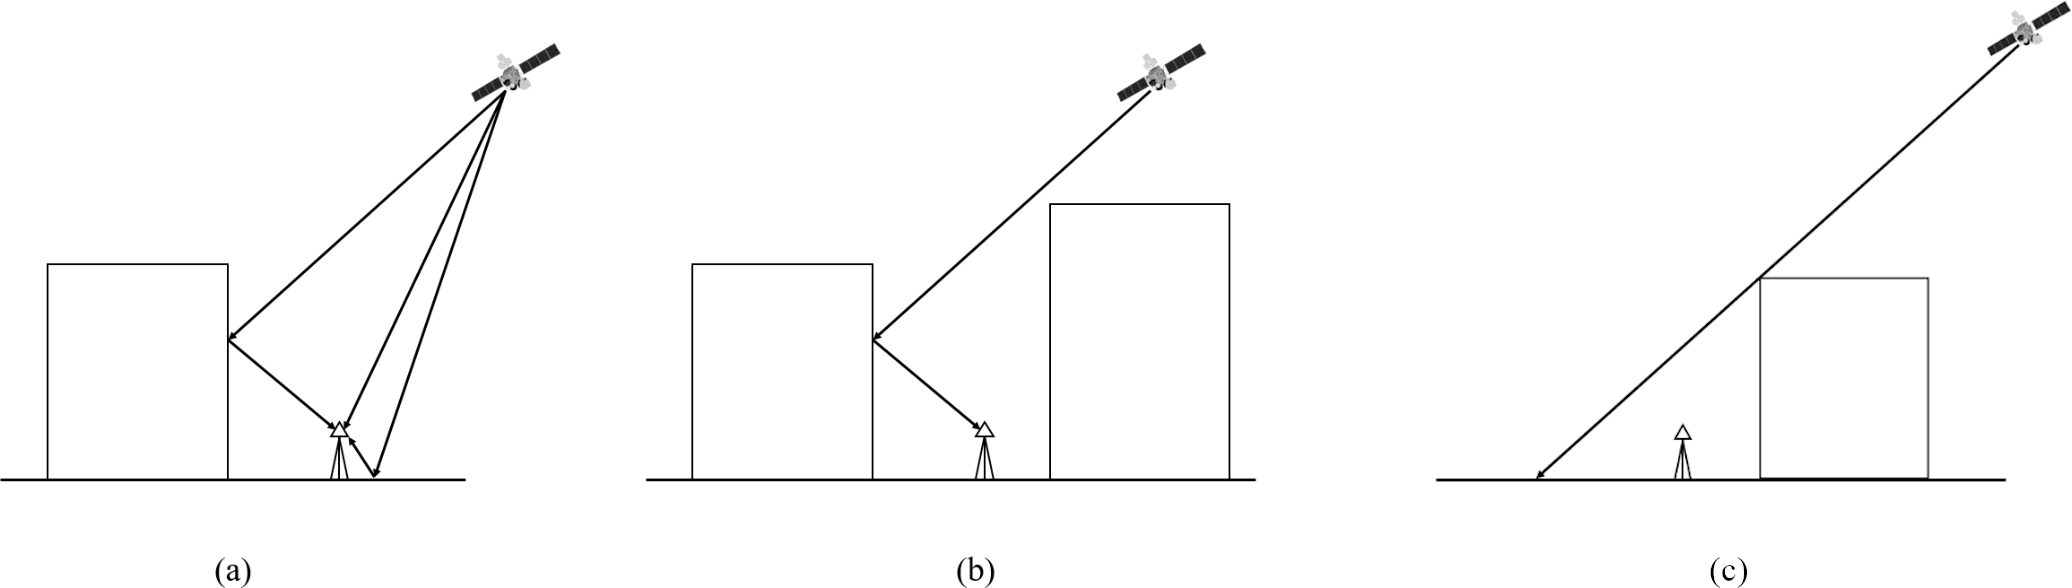
\includegraphics[width=0.9\textwidth]{fig/signal-paths.png}    
\caption{Возможные пути сигнала от спутника до приёмника \cite{Seeber2003}.}
\label{fig-signal-paths}      
\end{figure}

В некоторых случаях, например, как показано на рис. \ref{fig-signal-paths} (с), приёмник может быть полностью закрыт от всех прямых и отражённых сигналов.
Тем не менее из-за эффекта диффракции сигнал все равно будет поступать на приёмник.
Дифрагированный сигнал проходит намного более длинный путь, чем геометрическое расстояние между приёмником и спутником.
Таким образом, ошибка позиционирования может составлять от нескольких сантиметров до дециметров \cite{Seeber2003}.
Для устранения этого источника ошибки используются модели дифракционных эффектов (например, модель SIGMA-$\delta$ \cite{Brunner1999}).

Когда две волны накладываются в пространстве, их амплитуды в каждой точке суммируются.
Этот эффект называется интерференцией.
Существует два типа интерференции: конструктивная (когда максимум одной волны совпадает с максимумом другой волны, амплитуда результирующей волны увеличивается) и деструктивная (когда максимум одной волны совпадает с минимумом другой волны, амплитуда результирующей волны уменьшается).
При позиционировании особое значение имеет деструктивная интерференция, потому что она уменьшает отношение сигнал/шум (Signal-to-Noise Ratio, SNR).
Для избежания этой проблемы GPS использует методы расширения спектра, т.е. распределяет мощности сигналов в определённых полосах пропускания (2,046 МГц для C/A кода и 20,46 МГц для P кода).

\subsection*{\textbf{Аппаратные ошибки}}

Помимо ошибок часов спутника и приёмника существет ряд других аппаратных ошибок.
К ним относятся смещение фазового центра антенны, инструментальные ошибки и шум.

До сих пор полагалось, что антенны спутника и приёмника являются точечными.
В действительности же этого не так.
Поэтому возникает следующий вопрос: какую точку антенны следует использовать при измерении расстояния?
Эта точка называется фазовым центром антенны (Antenna Phase Center, APC).
Соответственно, расстояние между спутником и приёмником определяется, как расстояние между фазовыми центрами их антенн.
Смещение фазового центра антенны обычно составляет от миллиметров до сантиметров \cite{Seeber2003}.

При прохождении сигнала через комплектующие приёмника и спутника возникают так называемые инструментальные ошибки.
Эти ошибки отличаются для каждого типа измерений GPS и зависят от частоты сигнала.
Инструментальные ошибки могут быть смоделированы в общем виде следующи образом \cite{Xu2007}:
\begin{equation}
\begin{aligned}
&d_c=d_{c,i}(f)+d_c^j(f) \\
&d_p=d_{p,i}(f)+d_p^j(f) \\
&d_d=d_{d,i}(f)+d_d^j(f)
\end{aligned}    
\end{equation}
где
$f$ -- частота сигнала;
индексы $c$, $p$ и $d$ соответствуют кодовым, фазовым и доплеровским измерениям приёмника;
индексы $i$ и $j$ соответствуют номеру приёмника и спутника. 
Инструментальные ошибки могут быть устранены, например, путём использования метода относительного позиционирования.

Источники случайных ошибок выключают в себя помехи в кабелях, усилителях и антенне приёмника, тепловые шумы,  динамическое напряжение и т.д.
Полностью избежать шума невозможно, но для снижения его уровня можно использовать такие методы, например, как фильтрация нижних частот.
Современные приёмники способны уменьшить шумовую компоненту ошибки позиционирования вплоть до миллиметрового и ниже уровня \cite{Seeber2003}.

\subsection*{\textbf{Геометрия спутников}}

На точность позиционирования также влияет геометрическое расположение спутников, видимых приёмнику: чем больше спутники разнесены относительно друг друга в пространстве, тем лучше (ошибка меньше).
Для характеристики этого эффекта используется коэффициент DOP (Dilution Of Precision). 
Геометрическая интерпретация DOP для двумерного случая изображена на рис. \ref{fig-dop}. 
\begin{figure}[h]
\centering    
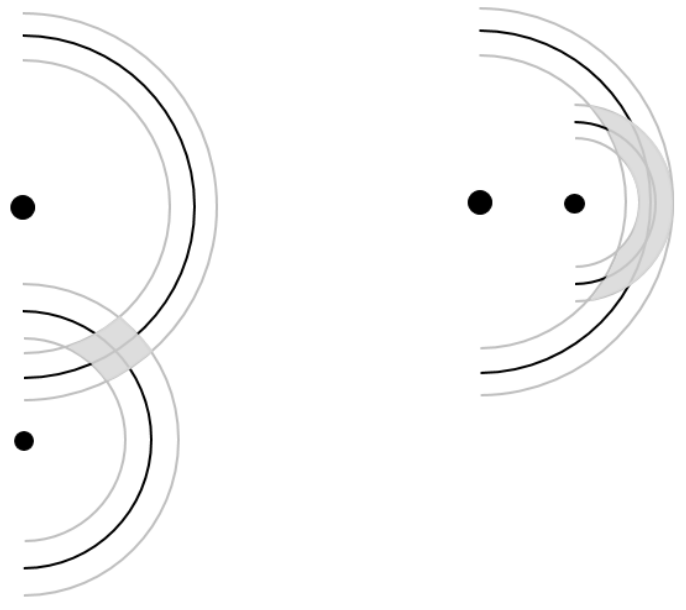
\includegraphics[width=0.3\textwidth]{fig/dop.png}    
\caption{Геометрическая интерпретация DOP \cite{Seeber2003}. Точками обозначены спутники, чёрные полуокружности представляют собой истинное расстояние до приёмника, а серые полуокружности -- расстояние с учётом погрешности.}
\label{fig-dop}      
\end{figure}

На значение DOP умножаются все остальные типы ошибок. 
В теоретическом идеальном случае DOP равен 1.
Однако на практике DOP редко бывает меньше 2, а в отдельны случаях может достигать даже 20 \cite{Sickle2001}.
DOP минимизируется самим приёмником путём выбора оптимальной комбинации видимых спутников.

\subsection*{\textbf{Другие источники ошибок}}

Выше были рассмотрены наиболее важные источники ошибок, но этот список не является полностью исчерпывающим.
Существует множество других физических эффектов, которые вносят небольшие ошибки в точность позиционирования.
Одним из таких эффектов является деформация земной коры под влиянием приливообразующих сил \cite{Subirana2013, Xu2007}. 